\documentclass[10pt]{extarticle}

\input{style}
\usepackage{cancel}
\usepackage{stackengine}
\usepackage{amsmath}
\usepackage{mathtools}
\usepackage{bm}
\usepackage{tikz}
\usepackage{pgfplots}
\usepackage{stmaryrd}
\usepackage{csquotes}
\usepackage{booktabs}
\usepackage{array} % put this in your preamble
\usepackage{adjustbox} % put this in your preamble
\pgfplotsset{compat=newest}
\usetikzlibrary{positioning,arrows.meta}
\usepgfplotslibrary{fillbetween}

\title{TAs' Notes - STAT-4300 Spring'26}
\date{\today}

\newcommand{\vtr}[1]{\bm{#1}} % or \bm
\newcommand{\mtr}[1]{\bm{#1}} % or \bm
\newcommand{\Var}{\mathbb{V}}
\newcommand{\symd}{\ \triangle\ }
\begin{document}

% \setlength{\abovedisplayskip}{3pt}
% \setlength{\belowdisplayskip}{3pt}
% \setlength{\abovedisplayshortskip}{0pt}
% \setlength{\belowdisplayshortskip}{0pt}

\maketitle
\newpage

%Custom colors for different environments
\definecolor{contcol1}{HTML}{72E094}
\definecolor{contcol2}{HTML}{24E2D6}
\definecolor{convcol1}{HTML}{C0392B}
\definecolor{convcol2}{HTML}{8E44AD}

\begin{tcolorbox}[
    title=Contents, 
    fonttitle=\huge\bfseries\selectfont,
    interior style={left color=contcol1!40!white,right color=contcol2!40!white},
    frame style={left color=contcol1!80!white,right color=contcol2!80!white},
    interior style={left color=blue!40!white, right color=cyan!40!white},
    frame style={left color=blue!80!white, right color=cyan!80!white},
        colbacktitle=contcol1!40!white, % highlight color behind Contents
        coltitle=black,
        top=2mm,bottom=2mm,left=2mm,right=2mm,breakable
]
\makeatletter
\@starttoc{toc}
\makeatother
\end{tcolorbox}

\newpage

\section{Class 1 - Set Theory, Probability, and Indicator Functions}

\subsection{Set Theory}

\subsubsection{Review of basic definitions}
We begin with definitions that should be familiar. 

\begin{definition}[Set]: A \textbf{set} is a collection of elements.
\end{definition}

\begin{definition}[Subset and superset]: A set $A$ is a \textbf{subset} of $B$ if every element of $A$ is also an element of $B$, denoted 
  \[
      A \subset B
  \]
  Equivalently, $B$ is a \textbf{superset} of $A.$
\end{definition}

\begin{definition}[Null set and empty set] The set with no elements is called the \textbf{null set} or the \textbf{empty set}, denoted $\emptyset$.
\end{definition}

\begin{remark}
  The null set is a subset of any set. I.e. for any $A$,
  \[
      \emptyset \subset A
  \]
\end{remark}

\begin{definition}
  (Universal set): The \textbf{universal set} is the set of all things that we could possibly consider in the context we are studying. 
\end{definition}

\begin{remark}
  In probability, the universal set is typically the sample space denoted $\Omega$
\end{remark}

\subsubsection{Review of set operations}
Except for \textbf{symmetric difference}, most of these set operations should be familiar.

\begin{definition}[Union]: The \textbf{union} of two sets, $A$ and $B$, is a set containing all the elements that are in $A$ or in $B$ (possibly both). \\

  The union of two sets, $A$ and $B$ is denoted 
  \[
  A \cup B
  \]
  The union of three or more sets, say $A_1, A_2, \hdots A_n$ is denoted 
  \[
      A_1 \cup A_2 \cup A_3 \hdots \cup A_n = \bigcup_{i = 1}^n A_i
  \]
\end{definition}

\begin{definition}
  [Intersection]: The \textbf{intersection} of two sets, $A$ and $B$, is a set containing all the elements that are both in $A$ and $B$. \\

  The intersection of two sets, $A$ and $B$ is denoted 
  \[
  A \cap B
  \]
  The intersection of three or more sets, say $A_1, A_2, \hdots A_n$ is denoted 
  \[
      A_1 \cap A_2 \cap A_3 \hdots \cap A_n = \bigcap_{i = 1}^n A_i
  \]
\end{definition}

\begin{definition}
  [Complement]: The \textbf{complement} of a set $A$ denoted by $A^C$ is the set of all elements that are in the universal set $S$ but are not in $A$.
\end{definition}

\begin{definition}
  [Difference, subtraction of sets]: The \textbf{difference} of two sets is defined where $A - B$ consists of the elements that are in $A$ but not in $B$. This is denoted
  \[
      A - B = A \setminus B = \{ x \in \Omega: x \in A, x \notin B \} 
  \]
\end{definition}

\begin{remark}
  From the above definition, it should be clear that 
  \[
      A - B = A \cap B^C
  \]
\end{remark}

\begin{definition}
  [Mutually exclusive, disjoint]: Two sets, $A$ and $B$, are \textbf{mutually exclusive} or \textbf{disjoint} if they do not have any shared elements, i.e. 
  \[
      A \cap B = \emptyset
  \]
\end{definition}

For three or more sets, the sets having a trivial intersection does not mean they are disjoint. Instead, we require the stronger condition below.

\begin{definition}
  [Pairwise disjoint]: Several sets are \textbf{pairwise disjoint} if no two sets share a common element.
\end{definition}

% \begin{definition}
%   (Partition): We say that a collection of nonempty sets $A_1, A_2, \hdots$ form a \textbf{partition} of $A$ if they are disjoint and their union is $A$.
% \end{definition}


\subsubsection{Review of common set properties}

\begin{theorem}
  (De Morgan's law): For sets $A_1, A_2, \hdots A_n$, we have 
  \begin{itemize}
      \item $ \left( A_1 \cup A_2 \cup \hdots A_n \right)^C = A_1^C \cap A_2^C \cap \hdots A_n^C $
      \item $ \left( A_1 \cap A_2 \cap \hdots A_n \right)^C = A_1^C \cup A_2^C \cup \hdots A_n^C $
  \end{itemize} 
\end{theorem}

\begin{theorem}
  (Distributive law): For any sets $A, B, C$, we have 
  \begin{itemize}
    \item $A \cap (B \cup C) = (A \cap B) \cup (A \cap C)$
    \item $A \cup (B \cap C) = (A \cup B) \cap (A \cup C)$
  \end{itemize}
\end{theorem}

\subsubsection{The symmetric difference}
Pay especially close attention to the symmetric difference, which may not have been emphasized upon in previous courses.

\begin{definition}
  [Symmetric difference]: The \textbf{symmetric difference} of two sets, $A$ and $B$, is defined as the set of elements that are only in $A$ or in $B$, but not both. This is denoted
  \[
  A \symd B
  \]

  The symmetric difference of two sets is their union, minus their intersection 
  \[
      A \symd B = (A \cup B) \setminus (A \cap B)
  \]
\end{definition}

\begin{result}
  Properties of the symmetric difference
  \begin{enumerate}
      \item Commutativity
      \[
      A \symd B = B \symd A
      \]
      \item Associativity
      \[
      (A \symd B) \symd C = A \symd (B \symd C)
      \]
      \item Distributivity of the intersection 
      \[
          A \cap \left( B \symd C \right)  = \left( A \cap B \right)  \symd (A \cap C)
      \]
      \item The symmetric difference is trivial if and only if the two sets are equal 
      \[
          A \symd B = \emptyset \iff A = B
      \]
      \item Taking complement with respect to the same universal set, 
      \[
      A \symd B = A^C \symd B^C
      \]
      \item The symmetric difference is a subset of the union
      \[
      A \symd B \subseteq A \cup B
      \]
      \item The symmetric difference is equal to the union if and only if the sets are disjoint 
      \[
      A \symd B = A \cup B \iff A \cap B = \emptyset
      \]
      \item The symmetric difference and the intersection partition the union, since
      \begin{align*}
          & (A \symd B) \cap (A \cap B) = \emptyset  \\
          & (A \symd B) \cup (A \cap B) = A \cup B
      \end{align*}
      \textit{The concept of partition will be introduced in Class 2}
      \item We can define the union using 
      \[
          A \cup B = (A \symd B) \symd (A \cap B)
      \]
  \end{enumerate} 
\end{result}

The following result is especially important. Hence we discuss it separately. 

\begin{lemma}
  \label{lem:symm-diff-union}
  Given arbitrary sets $A_1, A_2, \hdots A_n$ and $B_1, B_2, \hdots B_n$, 
  \begin{align*}
    \left( \bigcup_{i = 1}^n A_i \right)  \symd \left( \bigcup_{i = 1}^n B_i \right)  \subseteq \bigcup_{i = 1}^n \left( A_i \symd B_i \right) 
  \end{align*}
\end{lemma}

The proof of this lemma is revisited later in the lecture after the introduction of indicator functions. We will see that the proof is simple once we introduce indicators.

\subsection{Probabilities}

\subsubsection{Review}

\begin{definition}
  [Random experiment, outcome, sample space]: 
  \begin{itemize}
      \item A \textbf{random experiment} is a process by which we observe something uncertain.
      \item The result of a random experiment is an \textbf{outcome}. 
      \item The set of possible outcomes is the sample space.
  \end{itemize} 
\end{definition}

\begin{definition}
  [Event]: An \textbf{event} $E$ is a subset of the sample space, i.e. a collection of outcomes.
\end{definition}

\begin{remark}
  If $A$ and $B$ are events, then $A \cup B$ and $A \cap B$ are also events. \\

  $A \cup B$ occurs if $A$ \textbf{or} $B$ occurs. \\

  $A \cap B$ occurs if $A$ \textbf{and} $B$ occurs. \\
\end{remark}

\begin{definition}
  [Probability]: The \textbf{probability} measure of event $A$ is denoted $P(A)$.
\end{definition}


\subsubsection{Axioms of probability}
\begin{definition}
  [Axioms of probability]: The axioms of probability state that 
  \begin{enumerate}
      \item For any event $A$, $P(A) \geq 0$
      \item Probability of the sample space $\Omega$ is $P(\Omega) = 1$
      \item If $A_1, A_2, A_3 \hdots$ are disjoint, then 
      \[
      P(A_1 \cup A_2 \cup A_3 \hdots) = P(A_1) + P(A_2) + P(A_3) + \hdots
      \]
  \end{enumerate} 
\end{definition}

\subsubsection{Inclusion-Exclusion Principle}

\begin{result}
  [Inclusion-exclusion]: By the \textbf{inclusion-exclusion principle}, we have 
  \[
  P(A \cup B) = P(A) + P(B) - P(A \cap B)
  \]
  In general for $n$ events $A_1, \hdots A_n$, 
  \begin{align*}
  P \left( \cup_{i =1}^n A_i \right)  &= \sum\limits_{i = 1}^{n}  P(A_i) \\
& - \sum\limits_{i < j}^{}  P(A_i \cap A_j) \\
& + \sum\limits_{i < j < k}^{}  P(A_i \cap A_j \cap A_k) \\
& \vdots \\
& + (-1)^{n-1} P\left(\bigcap_{i = 1}^n A_i\right) \\
  \end{align*}
\end{result}



\subsection{Indicator Functions}

\subsubsection{Definition}

\begin{definition}
  [Indicator function]: Given an arbitrary set $X$, and a subset $A \subseteq X$, the \textbf{indidcator function} of $A$ is 
  \[
  \bm{1}_A(x) = \begin{cases}
    1 \text{ if } x \in A \\
    0 \text{ if } x \notin A
  \end{cases}
  \]
\end{definition}

\subsubsection{Properties of the indicator function}

\begin{result}
  Properties of the indicator function 
  \begin{enumerate}
    \item Indicator of the intersection is the product of indicators
    \[
    \bm{1}_{A \cap B} (x) = \min \{ \bm{1}_A(x), \bm{1}_B(x) \} = \bm{1}_A(x) \cdot \bm{1}_B(x)
    \]
    \item Ihe indicator of the union is sum of indicators minus their product
    \begin{align*}
    \bm{1}_{A \cup B} (x) &= \max \{ \bm{1}_A(x), \bm{1}_B(x) \} \\
    & = \bm{1}_A(x) + \bm{1}_B(x) - \bm{1}_A(x) \cdot \bm{1}_B(x) \\
    & = \bm{1}_A(x) + \bm{1}_B(x) - \bm{1}_{A \cap B}(x) \\
    \end{align*}
    \item Indicator of the complement 
    \[
    \bm{1}_{A^C} = 1 - \bm{1}_A
    \]
    \item If $A, B$ disjoint 
    \begin{align*}
    \bm{1}_{A \cup B} &= \bm{1}_{A} + \bm{1}_B \\
    \bm{1}_{A \cap B} &= 0
    \end{align*}
    \item Indicators of subsets
    \[
    A \subseteq B \iff \bm{1}_A \leq \bm{1}_B
    \]
    \item Indicators of difference of subsets
    \begin{align*}
      \bm{1}_{A - B}
      &= \bm{1}_{A \cap B^C} \quad \text{by definition of set subtraction} \\
      &= \bm{1}_A \cdot \bm{1}_{B^C} \quad \text{by indicator of intersections} \\
      &= \bm{1}_A\bigl(1 - \bm{1}_B\bigr) \quad \text{by indicator of complement} \\
      &= \bm{1}_A - \bm{1}_{A \cap B} \quad \text{by indicator of intersections}
    \end{align*}
    \item Indicators of symmetric difference
    \begin{align*}
      \bm{1}_{A \symd B}
      &= \bm{1}_{(A \cup B) \setminus (A \cap B)}
        \quad \text{by definition of symmetric difference} \\[6pt]
      &= \bm{1}_{A \cup B} \cdot \bm{1}_{(A \cap B)^C}
        \quad \text{by definition of set subtraction} \\[6pt]
      &= \bm{1}_{A \cup B}\bigl(1 - \bm{1}_{A \cap B}\bigr)
        \quad \text{by indicator of complement} \\[6pt]
      &= \bigl(\bm{1}_A + \bm{1}_B - \bm{1}_{A \cap B}\bigr)
        \bigl(1 - \bm{1}_{A \cap B}\bigr)
        \quad \text{by indicator of union} \\[6pt]
      &= \bm{1}_A + \bm{1}_B - 2\,\bm{1}_{A \cap B}
        \quad \text{since } \bm{1}_{A \cap B}^2 = \bm{1}_{A \cap B} \\[6pt]
      &= \bigl|\bm{1}_A - \bm{1}_B\bigr|
    \end{align*}
  \end{enumerate}
\end{result}

\subsubsection{Demonstrating the usefulness of indicators}
Recall Lemma~\ref{lem:symm-diff-union}. Given arbitrary sets $A_1,\dots,A_n$ and $B_1,\dots,B_n$,
\[
\left( \bigcup_{i=1}^n A_i \right)
\symd
\left( \bigcup_{i=1}^n B_i \right)
\subseteq
\bigcup_{i=1}^n (A_i \symd B_i).
\]

We can prove this lemma by reducing the set inclusion to an inequality involving indicator functions.

\begin{proof}
  By property 1.23.5, it suffices to show 
\begin{equation*}
\bm{1}_{\left(\cup_{i=1}^n A_i\right)\symd\left(\cup_{i=1}^n B_i\right)}
\le
\bm{1}_{\cup_{i=1}^n (A_i \symd B_i)}
\end{equation*}

By property 1.23.7 (indicator of symmetric differences), the LHS can be written as
\[
\left|
\bm{1}_{\cup_{i=1}^n A_i}(x)
-
\bm{1}_{\cup_{i=1}^n B_i}(x)
\right|
\]

By property 1.23.2 (indicator of unions)
\[
\bm{1}_{\cup_{i=1}^n A_i}(x) = \max_{1 \le i \le n} \bm{1}_{A_i}(x),
\qquad
\bm{1}_{\cup_{i=1}^n B_i}(x) = \max_{1 \le i \le n} \bm{1}_{B_i}(x),
\]
Hence we get 
\begin{equation*}
\left|
\max_{1 \le i \le n} \bm{1}_{A_i}(x)
-
\max_{1 \le i \le n} \bm{1}_{B_i}(x)
\right|
\le
\bm{1}_{\cup_{i=1}^n (A_i \symd B_i)}(x)
\end{equation*}

We now prove this inequality by enumerating the possible values of the
right-hand side.

\medskip

\noindent
\textbf{Case 1:} RHS = 0
\begin{align*}
& \bm{1}_{\cup_{i=1}^n (A_i \symd B_i)}(x) = 0 \\
\implies  & x \notin A_i \symd B_i \text{ for all } i \\
\implies & \bm{1}_{A_i}(x) = \bm{1}_{B_i}(x) \text{ for all } i \\
\implies &  \max_{i} \bm{1}_{A_i}(x) = \max_{i} \bm{1}_{B_i}(x) \\
\implies & 
\left|
\max_{1 \le i \le n} \bm{1}_{A_i}(x)
-
\max_{1 \le i \le n} \bm{1}_{B_i}(x)
\right| = 0
\end{align*}
Hence the inequality holds.

\medskip

\noindent
\textbf{Case 2:} RHS = 1 

Since the LHS is the absolute value of the difference of indicators, it takes values $0$ or $1$, and this is a simple upper bound.

\medskip

In both cases, the inequality holds. Since this inequality is
equivalent to the desired set inclusion, the lemma follows.
\end{proof}
\newpage
\section{Class 2 - Conditional Probability, Independence, and Law of Total Probability}

\subsection{Conditional Probability}
% \begin{example}
%     [Motivating example: Polymarket] Let $\Omega_{world}$ be the sample space of all future states of the world. Each element of the sample space $\omega \in \Omega_{world}$ represents a possible future state of the world. \\ 

%     Let $A$ be the event that Trump acquires Greenland by 2027. \\

%     Traded contract: Binary contract on $A$. 
%     \begin{itemize}
%         \item if $\omega \in A$, contract pays \$1
%         \item otherwise, contract pays \$0
%     \end{itemize} 

%     Price of a share: $p = P(A)$ \\

%     Let $B$ be the event that Denmark wants to negotiate. We are interested in the probability of $A$ given $B$ has occured, i.e. $P(A | B)$. \\

%     The market reaction is an increase in price from $p = P(A)$ to $p_B = P(A | B)$.
% \end{example}

\begin{definition}
    [Conditional Probability] Let $A, B$ be events in a sample space $S$, with $P(B) > 0$, then the \textbf{conditional probability} of $A$ given $B$ is defined as 
    \[
        P(A | B) = \frac{P(A \cap B)}{P(B)}
    \]
\end{definition}

\begin{remark} 
    \textbf{Conditional probability is a probability}. Fix $B$, define $P_B( \cdot) = P( \cdot | B)$. Then, $P(\cdot | B)$ satisfies the three axioms of probability on the reduced sample space $B$.
    \begin{enumerate}
        \item Nonnegativity. For any $A$, $P(A | B) \geq 0$
        \item Normalized. $P(B | B) = 1$
        \item Countable additivity. If $A_1, A_2, A_3, \hdots$ disjoint, then 
        \[
            P(A_1 \cup A_2 \cup A_3 \hdots | B) = P(A_1 | B) + P(A_2 | B) + P(A_3| B) + \hdots
        \]
    \end{enumerate}
\end{remark}

\begin{proof}
    We verify the three axioms:
    \begin{enumerate}
        \item For any $A$, since $P(A \cap B) \geq 0$ and $P(B) > 0$, we have 
        \[
            P(A | B) = \frac{P(A \cap B)}{P(B)} \geq 0
        \]
        \item 
        \[
            P(B | B) = \frac{P(B \cap B)}{P(B)} = \frac{P(B)}{P(B)} = 1
        \]
        \item If $A_1, A_2, A_3, \hdots$ are disjoint, then 
        \begin{align*}
            P(A_1 \cup A_2 \cup A_3 \hdots | B) &= \frac{P((A_1 \cup A_2 \cup A_3 \hdots) \cap B)}{P(B)} \\
            &= \frac{P((A_1 \cap B) \cup (A_2 \cap B) \cup (A_3 \cap B) \hdots)}{P(B)} &&\text{(by distributing the intersection)}\\
            &= \frac{P(A_1 \cap B) + P(A_2 \cap B) + P(A_3 \cap B) + \hdots}{P(B)} &&\text{(by axiom 3 of probability)}\\
            &= P(A_1 | B) + P(A_2 | B) + P(A_3| B) + \hdots
        \end{align*}
    \end{enumerate}
\end{proof}

\begin{remark}
    In class, prof used a slightly different notation to prove countable additivity.
    \begin{align*}
        P_B \left( \bigcup_{i = 1}^n A_i \right) 
        &= \frac{
            P \left( B \cap \bigcup_{i = 1}^n A_i \right) 
        }{P (B)} \\ 
        &= \frac{
            P \left( \bigcup_{i = 1}^n (B \cap A_i) \right) 
        }{P(B)} \\
        &= \frac{
            \sum\limits_{i = 1}^{n}  P \left( B \cap A_i \right) 
        }{P(B)} \\
        &= \sum\limits_{i = 1}^{n}  P( A_i | B)
    \end{align*}
\end{remark}

% \begin{example}
%     [Rolling a die] Roll a fair six-sided die twice. What is the probability of getting at least a 3 given the sum is 6?  \\
    
%     Solution: The sample space is 
%     \[
%         \Omega = \{ 1, 2, \hdots 6 \}^2
%     \]

%     Define two events 
%     \begin{align*}
%         A &= \{  \text{at least one die shows 3} \}  \\
%         B &= \{ \text{the sum is 6} \} 
%     \end{align*}

%     What is $P(A | B)$? \\

%     The number of outcomes in $B \cap \Omega$ is 5
%     \[
%         B \cap \Omega = \{ (1, 5), (5, 1), (2, 4), (4, 2), (3, 3) \} 
%     \]

%     The number of outcomes in $A \cap B$ is 1
%     \[
%         A \cap B = \{ (3, 3) \}
%     \]

%     Therefore, 
%     \[
%         P(A | B) = \frac{1}{5}
%     \]

% \end{example}

\subsection{Independence}

% \begin{example}[Motivating example: new information does not change the market] Define 
%     \begin{align*}
%         A &= \{ \text{Trump acquires Greenland by 2027} \} \\
%         B &= \{ \text{It's raining in Nuuk} \}
%     \end{align*}

%     Then it might make sense to say that observing $B$ does not provide more information about $A$, i.e.
%     \[
%         P (A | B) = P(A)
%     \]
% \end{example}

\begin{definition}[Independence]
    Events $A, B$ are \textbf{independent} if and only if
    \[
        P(A \cap B) = P(A) P(B)
    \]

    Equivalent 
    \begin{align*}
        P(A | B) &= \frac{P(A \cap B)}{P(B)} \\
        &= \frac{P(A) P(B)}{P(B)} \\
        &= P(A)
    \end{align*}

    Independence is sometimes denoted 
    \[
        A \cap B
    \]
\end{definition}

\begin{remark} 
    [Independence vs Disjointness] 
    Two events are \textbf{disjoint} if $A \cap B = \emptyset$. \\

    Two events are independent if $P(A \cap B) = P(A) P(B)$ or $P(A|B) = P(A)$ \\

    If two events are disjoint (and each event has non-zero probability), knowing one event provides full information about the other. Therefore, disjoint events are \textbf{not} independent. 
\end{remark}

\begin{result}[Independence and complements] 
    Suppose $A, B$ are independent events. Then the following pairs of events are also independent:
    \begin{itemize}
        \item $A^c$ and $B$
        \item $A$ and $B^c$
        \item $A^c$ and $B^c$
    \end{itemize}
\end{result}

\subsection{Law of Total Probability}

% \begin{example}[Motivating example: Trump and cases]
%     Let 
%     \begin{align*}
%         A &= \{ \text{Trump acquires Greenland by 2027} \} 
%     \end{align*}

%     Break the future into two cases: 
%     \begin{align*}
%         B_1 &= \{ \text{Trump visits Nuuk} \} \\
%         B_2 &= \{ \text{Trump does not visit Nuuk} \}
%     \end{align*}

%     Suppose we know $P(B_1), P(B_2)$. 
%     \begin{itemize}
%         \item If $B_1$ occurs, then $P(A)$ updates to $P(A |B_1)$
%         \item If $B_2$ occurs, then $P(A)$ updates to $P(A |B_2)$
%     \end{itemize} 
    
%     Then, the probability of $A$ is a weighted sum of the conditional probabilities, weighted by $P(B_1), P(B_2)$. 
%     \[
%         P(A) = P(A | B_1) P(B_1) + P(A |B_2) P(B_2)
%     \]
    
% \end{example}


\begin{definition}
  [Partition] We say that a collection of nonempty sets $A_1, A_2, \hdots$ form a \textbf{partition} of $A$ if they are disjoint and their union is $A$.  \\
  
  That is, 
    \begin{itemize}
        \item pairwise disjoint: $A_i \cap A_j = \emptyset$ for all $i \neq j$
        \item collectively exhaustive: $\bigcup\limits_{i}^{} A_i = A$
        \item nonempty: $A_i \neq \emptyset$ for all $i$
    \end{itemize}
\end{definition}

\begin{remark} If $A_1, A_2, \hdots$ parition $\Omega$, then any $\omega \in \Omega$ lives in exactly one of the $A_i$'s.
\end{remark}


\begin{theorem}[Law of Total Probability]
    If $B_1, B_2, \hdots$ is a partition of the sample space $S$, then for any event $A$, we have 
    \begin{align*}
        P(A) &= \sum\limits_{i}^{} P(A \cap B_i) = \sum\limits_{i}^{} P(A | B_i) P(B_i)
    \end{align*}
\end{theorem}

\begin{proof}
    Decompose $A$ into disjoint unions and apply axiom 3.
    \begin{align*}
        A &= \bigcup_{i = 1}^n \left( A \cap B_i \right) \text{ and union is disjoint} \\
        P(A) &= P \left( \bigcup_{i = 1}^n \left( A \cap B_i \right) \right) \\
        &= \sum\limits_{ i= 1}^{n}  P(A \cap B_i) \quad \text{(by axiom 3)} \\
        &= \sum\limits_{ i= 1}^{n}  P(A | B_i) P(B_i)
    \end{align*}

\end{proof}




\newpage
\section{Class 3 - Law of total probability and Bayes Rule}

\newpage
\section{Class 4 - Multinomial Coefficients and Discrete Random Variables}

\subsection{Multinomial Coefficients}

\begin{definition}[Multinomial coefficient]
Let $S$ be a finite set with $|S|=n$.  
For nonnegative integers $m_1,\dots,m_n$ satisfying
\[
\sum_{i=1}^n m_i = k,
\]
the \textbf{multinomial coefficient}
\[
\binom{k}{m_1,\dots,m_n} = \frac{k!}{m_1!\cdots m_n!}
\]
counts the number of ordered sequences in $S^k$ in which element $i\in S$
appears exactly $m_i$ times.
\end{definition}

\begin{example}[Most likely outcome of 60 dice rolls]
    Roll a fair 6-sided die 60 times. Count the number of 1s, 2s, 3s, 4s, 5s, and 6s. What is the most likely unordered outcome? \\

    Let $\Omega = \{ 1, 2, \hdots 6 \}^{60} $. Each ordered outcome is equally likely. The most likely unordered outcome is the one where each element appears exactly 10 times. The number of such outcomes is given by the multinomial coefficient
    \[
        \binom{60}{10, 10, 10, 10, 10, 10} = \frac{60!}{(10!)^6}
    \]

    \textbf{Proof}:  Suppose two of the multiplicities differ by more than 1, i.e. $m_a \geq m_b + 2$ for some $a, b$. Then define
    \[
        m_a^{\prime} = m_a - 1, \quad m_b^{\prime} = m_b + 1
    \]

    We then compare the ratio of the two multinomial coefficients:
    \[
    \frac{
        \binom{60}{ \hdots m_a^{\prime}, \hdots, m_b^{\prime}, \hdots}
    }{
        \binom{60}{ \hdots m_a, \hdots, m_b, \hdots}
    } = \frac{
        m_a
    }{m_b + 1} > 1
    \]

    This means we can always increase the multinomial coefficient by balancing the multiplicities. Hence the maximum occurs when all multiplicities are within 1 apart.
\end{example}

\subsection{Discrete Random Variables}

\subsubsection{Discrete Random Variables, PMF, CDF}


\begin{definition}[Discrete random variables]
    A \textbf{discrete random variable} is a function $X: \Omega \to A \subseteq  \mathbb{R}$ where $A$ is countable (i.e. there is a one-to-one mapping between $A$ and $\mathbb{N}$, $ \left| A \right|  \leq \left| \mathbb{N} \right| $).
\end{definition}

\begin{remark}
    For discrete $X$, $\Omega$ can be arbitrarily complicated, but the range of $X$, $A$ needs to be countable.
\end{remark}


\begin{definition}[Probability mass function]
    The \textbf{probability mass function} (pmf) of a discrete random variable $X$ is the function $p_X: \mathbb{R} \to [0, 1]$ defined by
    \[
        p_X(x) = P(X = x) = P( \{ \omega \in \Omega: X(\omega) = x \} )
    \]
\end{definition}

\begin{definition}[Support]
    The \textbf{support} of a discrete random variable $X$ is the set of values in $\mathbb{R}$ where the pmf is positive: 
    \[
        \text{supp}(X) = \{ x \in \mathbb{R} : p_X(x) > 0 \}
    \]
\end{definition}


\begin{remark}
    The pmf satisfies
    \begin{itemize}
        \item $p_X(x) \geq 0$ for all $x \in \mathbb{R}$
        \item $\sum\limits_{x \in A}^{} p_X(x) = 1$, where $A$ is the range of $X$ 
    \end{itemize} 
\end{remark}

\begin{definition}[Cumulative distribution function]
    The \textbf{cumulative distribution function} (cdf) of a discrete random variable $X$ is the function $F_X: \mathbb{R} \to [0, 1]$ defined by
    \[
        F_X(t) = P(X \leq t) = \sum\limits_{a \leq t}^{} p_X(a)
    \]
\end{definition}

\begin{example}[Sum of two dice rolls]
    Let $D_1, D_2 \in \{ 1, 2, \hdots 6 \} $ be outcomes of 2 dice rolls. Define 
    \[
        S:= D_1 + D_2 \in A = \{ 2, 3, \hdots 12 \} 
    \]
    The sample space is 
    \[
        \Omega = \{ 1, 2, \hdots 6  \}^2
    \]

    The number of outcomes corresponding to sum $s$ is 
    \[
        N(s) = \begin{cases}
            s - 1 & \text{ if } 2 \leq s \leq 7 \\
            13 - s & \text{ if } 8 \leq s \leq 12
        \end{cases}
    \]
    The probability mass function of $S$ is
    \[
        p_S(s) = \frac{N(s)}{ \left| \Omega \right| } = \frac{N(s)}{36}
    \]
    
\end{example}

\subsubsection{Expectations and Variance}

\begin{definition}[Expectation of discrete random variable]
    If $X$ is a discrete random variable with pmf $p_X$, and $\sum\limits_{x \in A}^{}  \left| x \right| p_X(x) < \infty$, then the \textbf{expectation} of $X$ is defined as 
    \[
        \mathbb{E}\left[ X\right]  = \sum\limits_{ x \in \operatorname{supp}(X)}^{} x \cdot p_X(x)
    \]

    If $g: \mathbb{R} \to \mathbb{R}$, then the \textbf{expectation} of $g(X)$ is defined as
    \[
        \mathbb{E}\left[ g(X)\right]  = \sum\limits_{ x \in \operatorname{supp}(X)}^{} g(x) \cdot p_X(x)
    \]
\end{definition}

\begin{definition}[Variance]
    Given a random variable $X$ with finite expectation, the \textbf{variance} of $X$ is defined as
    \[
        \operatorname{Var}(X) = \mathbb{E}\left[ (X - \mathbb{E}\left[ X\right] )^2 \right]  = \mathbb{E}\left[ X^2 \right]  - ( \mathbb{E}\left[ X\right] )^2
    \]
\end{definition}


\subsubsection{Indicator random variables}

\begin{definition}[Indicator random variables] For an event $A \subseteq \Omega$, the \textbf{indicator function} is a discrete random variable $\bm{1}_A : \Omega \to \{ 0, 1 \} $ defined by 
    \[
        \bm{1}_A(\omega) = \begin{cases}
            1 & \text{ if } \omega \in A \\
            0 & \text{ if } \omega \notin A
        \end{cases}
    \]
\end{definition}

\begin{result}[Expectation of indicator r.v.]
    The expectation of an indicator random variable is the probability of the corresponding event:
    \[
        \mathbb{E}\left[ \bm{1}_A \right] = P(A)
    \]
\end{result}

\begin{proof}
    By definition of expectation 
    \begin{align*}
        \mathbb{E}\left[ \bm{1}_A \right] &= 1 \cdot P( \bm{1}_A = 1) + 0 \cdot P( \bm{1}_A = 0) \\
        &= P(A)
    \end{align*}
\end{proof}

\begin{theorem}[Linearity of Expectation]
    Let $X, Y$ be discrete random variables, and $a, b$ be constants, then 
    \[
        \mathbb{E}\left[ a X + bY \right]  = a \mathbb{E}\left[ X\right]  + b \mathbb{E}\left[ Y\right] 
    \]
\end{theorem}

\begin{remark}
    In general, $\mathbb{E}\left[ g(X)\right]  \neq g( \mathbb{E}\left[ X\right] )$.
\end{remark}

\begin{theorem}[Law of total probability] 
    Let $A_1, \hdots A_n$ be a partition of $\Omega$, define a discrete random variable $I : \Omega \to \{ 1, 2, \hdots n \}$  by 
    \[
        I(w) = i \text{ if } w \in A_i
    \]

    Then 
    \[
        P(I = i) = P(A_i)
    \]

    Define $g(I): P(B | I = i)$. Then the law of total probability can be stated as 
    \[
        P(B) = \sum\limits_{i = 1}^{n} P(B | A_i) P(A_i) = \mathbb{E}\left[ P(B | I)\right] 
    \]
    
\end{theorem}











\newpage

\section{Class 5 - Independence, Chebyshev's, Bernoullis, and Binomials}

\subsection{Independence of Random Variables}

We previously introduced independence of events. We now discuss independence of random variables.

\begin{remark}
    We use the following notational short hand
    \[
    P(X = x, Y = y) = P( \{ X = x \} \cap \{ Y = y \}  )
    \]
\end{remark}


\begin{definition}[Independence]
    Let $X, Y$ be discrete random variables on $\Omega$. We say that $X$ and $Y$ are \textbf{independent} if 
    \[
        P(X = x, Y = y) = P( \{ X = x \} \cap \{  Y = y \}  )  = P(X = x) P(Y = y)
    \] for every $x$ and $y$.
\end{definition}

\begin{result}[Expectation of product of independent random variables]
    Let $X, Y$ be discrete random variables on $\Omega$ with $\operatorname{supp}(X) = A , \operatorname{supp}(Y)  = B$. If $X, Y$ independent, then 
    \[
        \mathbb{E}\left[ XY\right]  = \mathbb{E}\left[ X\right] \mathbb{E}\left[ Y\right] 
    \]

    This is denoted
    \[
    X \perp Y
    \]
\end{result}

\begin{proof}
    \begin{align*}
        \mathbb{E}\left[ XY\right]  
        &= \sum\limits_{x \in A}^{}  \sum\limits_{y \in B}^{}  x \cdot y P (X = x, Y = y) \quad \text{ by definition of expectation} \\
        &= \sum\limits_{x \in A}^{}  \sum\limits_{y \in B}^{}  x \cdot y P (X = x) P(Y = y) \quad \text{ by independence} \\
        &= \left( \sum\limits_{ x \in A}^{}x P(X = x)  \right)  \left( \sum\limits_{y \in B}^{}y P(Y = y)  \right)  \\
        &= \mathbb{E}\left[ X\right]  \mathbb{E}\left[ Y\right]  \text{ by definition of expectation}
    \end{align*}
\end{proof}

\begin{remark}
    Note that the implication only works one way 
    \[
    X \perp Y \implies \mathbb{E}\left[ XY\right]  = \mathbb{E}\left[ X\right]  \mathbb{E}\left[ Y\right] 
    \]
    The converse is not true 
    \[
        \mathbb{E}\left[ XY\right]  = \mathbb{E}\left[ X\right]  \mathbb{E}\left[ Y\right] \not \Rightarrow X \perp Y 
    \]
    
\end{remark}

\subsection{Chebyshev's Inequality}

Chebyshev's allows us to bound the probability that a random variable deviates by a \textit{certain amount} from its mean.

\begin{theorem}[Chebyshev's Inequality]
    Let $X$ be a random variable with expectation $\mu$ and variance $\sigma^2$. For any $t > 0$,
    \[
    P \left(  \left| X - \mu \right| \geq t \right)  \leq \frac{\sigma^2}{t^2}
    \]
\end{theorem}

\subsection{Bernoulli Random Variable}

\begin{remark}
    For random variable $X$, we sometimes use the following short hand 
    \[
        P_X(x) = P(X = x)
    \]
\end{remark}


\begin{definition}[Bernoulli] 
    A random variable $X : \Omega \to \{ 0, 1 \} $ is a \textbf{Bernoulli} random variable with parameter $p \in [0, 1]$ if 
    \[
    P_X(1) = p, \quad P_X(0) = 1 - p
    \]
    We denote this 
    \[
        X \sim \operatorname{Bern} (p)
    \]
\end{definition}

\begin{result}[Moments of a Bernoulli random variable]

    The mean of a Bernoulli is  
    \[
    \mathbb{E}\left[ X\right]  = 1 \cdot p + 0 \cdot ( 1- p) = p
    \]

    To find $\mathbb{E}\left[ X^2\right] $
    \begin{align*}
        \mathbb{E}\left[ X^2\right]  &= \sum\limits_{x \in \{ 0, 1 \} }^{} x^2 P(X = x) \\
        &= 1 \cdot p + 0 \cdot ( 1-p) \\
        &= p
    \end{align*}
    

    The variance of a Bernoulli is 
    \begin{align*}
        \operatorname{Var} (X) &= \mathbb{E}\left[ X^2\right]  - \mathbb{E}\left[ X \right]^2 \\
        &= p - p^2
    \end{align*}
\end{result}

\begin{remark}
    The maximum variance of a Bernoulli random variable is achieved when $p = \frac{1}{2}$

\begin{center}
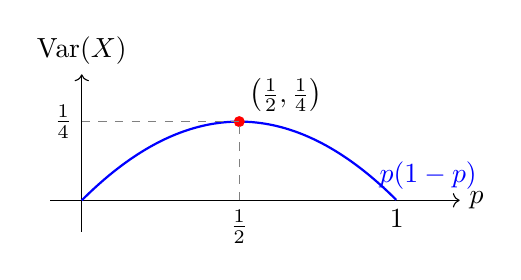
\begin{tikzpicture}[scale=4]
    % Axes
    \draw[->] (-0.1,0) -- (1.2,0) node[right] {$p$};
    \draw[->] (0,-0.1) -- (0,0.4) node[above] {$\operatorname{Var}(X)$};

    % Variance curve p(1-p)
    \draw[thick, blue, domain=0:1, samples=100] plot (\x, {\x*(1-\x)});

    % Maximum point at p = 1/2
    \fill[red] (0.5, 0.25) circle (0.5pt);
    \node[above right] at (0.5, 0.25) {$\left(\frac{1}{2}, \frac{1}{4}\right)$};

    % Dashed lines to axes
    \draw[dashed, gray] (0.5, 0) -- (0.5, 0.25);
    \draw[dashed, gray] (0, 0.25) -- (0.5, 0.25);

    % Tick marks
    \node[below] at (0.5, 0) {$\frac{1}{2}$};
    \node[below] at (1, 0) {$1$};
    \node[left] at (0, 0.25) {$\frac{1}{4}$};

    % Label for curve
    \node[blue] at (1.1, 0.08) {$p(1-p)$};
\end{tikzpicture}
\end{center}
\end{remark}

\subsection{Binomial Random Variable}

\begin{definition}
    [Binomial Random Variable]
    Let $X_1, \hdots X_n$ be independent Bernoullis with the same parameter $p \in [0, 1]$. A \textbf{binomial} random variable $S_n$ with parameter $n, p$ is defined as 
    \[
        S_n = \sum\limits_{i = 1}^{n} X_i
    \]
    $S_n$ takes as its support $\{  0, 1, \hdots n \} $. \\

    $S_n$ has pmf
    \[
    P(S_n = x) = \begin{cases}
        \binom{n}{x} p^x (1 - p)^{n - x} & \text{if } x \in \operatorname{supp}(S_n) \\
        0 & \text{otherwise}
    \end{cases}
    \]
    We denote this 
    \[
    S_n \sim \operatorname{Binom} (n, p)
    \]
\end{definition}

\begin{proof}
    We want to show for $x \in \operatorname{supp}(S_n) $,
    \[P(S_n = x) = \binom{n}{x} p^x (1-p)^{n-x}
    \]

    Fix $x \in \operatorname{supp}(S_n) $. An outcome with exactly $x$ successes is an unordered collection of $x$ successes and $n - x$ failures. Each ordered sequence with $x$ successes is equally likely. \\

    The probability of getting an ordered sequence of $x$ successes followed by $n-x$ failures is, by independence,
    \[
        p^x (1-p)^{n-x}
    \]
    The number of such sequences is the number of ways to choose $x$ positions in $n$ to be successes
    \[
        \binom{n}{x}
    \]

    Hence the pmf is
    \[
        P(S_n = x) = \binom{n}{x} p^x (1-p)^{n-x}
    \]
\end{proof}


\begin{remark}
    A binomial random variable with parameter $n, p$ counts the number of successes in $n$ independent and idential trials, each with success probability $p$.
\end{remark}

\begin{result}[Moments of Binomial random variables]
    The mean of a binomial random variable is 
    \begin{align*}
        \mathbb{E}\left[ S_n\right]  &= \mathbb{E}\left[ 
            \sum\limits_{i = 1}^{n}  X_i
        \right] \quad \text{by definition}\\
        &= \sum\limits_{i = 1}^{n}  X_i \quad \text{by linearity of expectation} \\
        &= \sum\limits_{i = 1}^{n}  p \\
        &= np
    \end{align*}
    To find $\mathbb{E}\left[ S_n^2\right] $
    \begin{align*}
        \mathbb{E}\left[ S_n^2\right] &= \mathbb{E}\left[ 
            \left( \sum\limits_{i = 1}^{n} X_i \right)^2 
        \right]  \\
        &= \mathbb{E}\left[ 
            (X_1 + X_2 + \hdots X_n)^2
        \right]  \\
        &= \mathbb{E}\left[ 
            \sum\limits_{i = 1}^{n}  X_i^2 
            + 
            \sum\limits_{ i \neq j}^{}  X_i X_j
        \right] \\
        &= \sum\limits_{i = 1}^{n}  \mathbb{E}\left[ X_i^2\right]  + \sum\limits_{i \neq j}^{}  \mathbb{E}\left[X_i X_j \right] \quad \text{by linearity} \\
        &= \sum\limits_{i = 1}^{n}  \mathbb{E}\left[ X_i^2\right]  + \sum\limits_{i \neq j}^{}  \mathbb{E}\left[X_i \right] \mathbb{E}\left[ X_j\right]  \quad \text{by independence of $X_i, X_j$} \\ 
        &= \sum\limits_{i = 1}^{n} p  + \sum\limits_{i \neq j}^{} p^2\\
        &= np + n(n-1) p \\
    \end{align*}

    Hence the variance of $S_n$ is 
    \begin{align*}
        \operatorname{S_n}  &= \mathbb{E}\left[ S_n^2\right]  - \mathbb{E}\left[ S_n\right]^2 \\
        &= np + n(n-1)p - (np)^2 \\
        &= np(1-p)
    \end{align*}
\end{result}

\begin{remark}
    To see how we expand $(X_1 + X_2 + \hdots + X_n)^2$, consider the multiplication table:
    \[
    \begin{array}{c|cccc}
         \times & X_1 & X_2 & \cdots & X_n \\
        \hline
        X_1 & \boxed{X_1^2} & X_1 X_2 & \cdots & X_1 X_n \\
        X_2 & X_2 X_1 & \boxed{X_2^2} & \cdots & X_2 X_n \\
        \vdots & \vdots & \vdots & \ddots & \vdots \\
        X_n & X_n X_1 & X_n X_2 & \cdots & \boxed{X_n^2}
    \end{array}
    \]

    The sum of all entries in this $n \times n$ table gives $(X_1 + \hdots + X_n)^2$:
    \begin{itemize}
        \item {Diagonal entries}: $n$ terms
        \item {Off-diagonal entries}: $n(n-1)$ terms, there are a few ways to see this
        \begin{itemize}
            \item $n^2 - n$ terms, by counting total terms - $n$ diagonal terms 
            \item ${}_n P_2$ terms, by counting number of ways to permute $2$ out of $n$ 
            \item $2 \cdot {}_n C_2 = 2 \binom{n}{2}$ terms, by counting number of ways to choose $2$ out of $n$ terms, and then permuting the 2 terms
        \end{itemize} 
    \end{itemize}

    Hence
    \[
        (X_1 + X_2 + \hdots + X_n)^2 = \underbrace{\sum_{i=1}^{n} X_i^2}_{n \text{ terms}} + \underbrace{\sum_{i \neq j} X_i X_j}_{n(n-1) \text{ terms}}
    \]
\end{remark}

\begin{remark}[Concentration of binomial]
    Let $S_n \sim \operatorname{Binom}(n, p) $

    \textbf{Intuition}: For a binomial \textit{most probability mass lies near the center}. \\

    When $p = \frac{1}{2}$
    
    \[P(S_n = k) = \binom{n}{k} \left( \frac{1}{2}\right)^{k} \left(\frac{1}{2}\right)^{n - k} = \binom{n}{k} 2^{-n}
    \]

    The binomial coefficient is biggest when $ k = \frac{k}{2}$
    
    We can quantify the extent to which the pmf \textit{concentrates around the center} this using mean, variance, and Chebyshev's. \\

    \textbf{Proof}: \\

    By Chebyshev's, for any positive $t$ 
    \begin{align*}
        P \left( \left| S_n - np \right| \geq t  \right)  \leq \frac{np(1-p)}{t^2}
    \end{align*}

    This inequality is not very meaningful is $n$ is very large and $t$ is small, in which case our LHS will be something bigger than 1. We already know for free that the probability is less than 1.\\

    Since we get to choose whatever $t$ we want, we pick a $t$ such that $t^2$ is \textit{roughly as big as} $n$. \\

    Pick $t^2 = c\cdot n$. Then 
    \begin{align*}
        P \left( \left| S_n - np \right| \geq \sqrt{ c \cdot n} \right)  \leq \frac{p (1-p)}{c}
    \end{align*}

    \textbf{Conclusion}: Deviations of $S_n$ on the order of $\sqrt{n}$ happens with non-neglegible probability.  \\

    \textbf{Example}: Say $p = \frac{1}{2}$, then $S_n$ deviates from $ \frac{n}{2}$ by about $ \frac{\sqrt{n}}{2}$
    \begin{itemize}
        \item $n = 100, \frac{\sqrt{n}}{2} = 5$, most outcomes will be in $[45, 55]$
        \item $n = 10,000, \frac{\sqrt{n}}{2} = 50$, most outcomes will be in $[4950, 5050]$
    \end{itemize} 

    In the symmetric case ($p = \frac{1}{2}$), 
    \[
    P \left( \left| S_n - \frac{n}{2} \right|  \geq t \right)  \leq \frac{n}{4t^2}
    \]
    Take $t = 5 \sqrt{n}$
    \[ 
    P \left( \left| S_n - \frac{n}{2} \right|  \geq 5 \sqrt{n} \right) \leq \frac{1}{100}
    \]
    \textit{For symmetric binomial, we have less than 1\% chance of seeing a deviation of more than $5 \sqrt{n}$}.
\end{remark}






\newpage
\section{Class 6 - Discrete Random Variables, PMFs, Expectation and Variance}

\newpage
\section{Class 7 - Pascal Random Variables and Coupon Collector Probelm}

\subsection{Pascal Random Variables}

\begin{definition}[Pascal random variable]
    A random variable $T_r$ is said to be a \textbf{Pascal} ranodm variable with parameters $r, p$, denoted $T_r \sim \operatorname{Pascal}(r, p) $ if its PMF is given by 
    \[
        P_{T_r}(k) = P (T_r = k) = \binom{k-1}{r-1} p^r (1-p)^{k-r}
    \]

    for $k = r , r+1, r+ 2, \hdots$, $p \in (0, 1)$.
    

\end{definition}

\begin{remark}
    A Pascal random variable, $T_r \in \operatorname{Pascal}(r, p)$ can be understood as the waiting time until we see exactly $r$ successes, where each identical trial has success probability $p \in (0, 1]$. \\
    
    $T_r$ takes as its support $\operatorname{supp}(T_r) = \{ r, r+1, r+2 \hdots \} $.  \\

    $T_r$ is the sum of $r$ iid geometric random variables. 
    \[
        T_r = \sum\limits_{i = 1}^{r} G_i, \quad G_i \sim \operatorname{Geom} (p)
    \]
    This gives us a much easier way to calculate its mean and variance, as shown below.
\end{remark}


\begin{result}[Moments of Pascal Random Variables]
    The expectation is 
    \[
        \mathbb{E}\left[ T_r\right]  = \mathbb{E}\left[  \sum\limits_{i = 1}^{r} G_i \right]  = \sum\limits_{i = 1}^{r} \mathbb{E}\left[ G_i \right]  = \frac{r}{p}
    \]

    The variance is 
    \[
        Var(T_r) = Var \left( \sum\limits_{i = 1}^{r} G_i \right)  = \sum\limits_{i = 1}^{r} Var (G_r) = \frac{r(1-p)}{p^2}
    \]
\end{result}

\subsection{Coupon Collector Problem}

The coupon collector problem is a classic waiting time problem. We now have a way to think about the mean, variance and concentration of the random variable that we want to study. \\

To think about what happens to the waiting time as the number of trials get large, we use the following notation.

\begin{definition}[Asymptotic tight bound, $\Theta$-notation]
    For a function $f(n)$, we say that a function $g(n)$ is an \textbf{asymptotically tight bound} for $f(n)$, or $f(n)$ is $\Theta(g(n))$, or $f(n) \in \Theta(g(n))$ if there exists positive constants $c_1, c_2, n_0$ such that for all $n \geq n_0$
    \[
        0 \leq c_1 g(n) \leq f(n) \leq c_2 g(n)
    \]
\end{definition}

% \begin{remark}
%     $g(n)$ is asymptotic tight bound of $f(n)$ if past a certain point, $f(n)$ gets sandwiched by scaled versions of $g(n)$.
%     \begin{center}
% \begin{tikzpicture}[scale=0.8]
%     \draw[thick,->] (0,0) -- (7.5,0) node[right, font=\large] {$n$};
%     \draw[thick,->] (0,0) -- (0,5.5);
    
%     \def\nzero{1.2}
%     \draw[dashed, gray, thick] (\nzero,0) -- (\nzero,5);
%     \node[below, font=\large] at (\nzero,-0.15) {$n_0$};
    
%     \draw[thick, domain=0:7, smooth, samples=100] 
%         plot (\x, {0.35*\x^1.2});
%     \node[right, font=\large] at (7.1, {0.35*7^1.2}) {$c_2g(n)$};
    
%     \draw[thick, domain=0:7, smooth, samples=150] 
%         plot (\x, {0.22*\x^1.2 + 0.12*exp(-0.8*\x)*sin(deg(5*\x))});
%     \node[right, font=\large] at (7.1, {0.22*7^1.2}) {$f(n)$};
    
%     \draw[thick, domain=0:7, smooth, samples=100] 
%         plot (\x, {0.12*\x^1.2});
%     \node[right, font=\large] at (7.1, {0.12*7^1.2}) {$c_1g(n)$};
% \end{tikzpicture}
%     \end{center}
% \end{remark}



\begin{example}[Coupon Collector Problem]
    Given $n$ distinct coupons. Let $T$ be the time it takes to see all $n$ coupons. \\

    $T$ is a sum of independent geometric random variables. \textbf{Unlike the Pascal random variable}, which is a sum of independent, identical geometric random variables, here the geometric random variables are \textbf{not identical}. \\

    Define $G_i$ to be the time taken to see the $i$-th new coupon. Then for $i \in \{ 1, 2, \hdots n \} $
    \begin{align*}
        G_1 & \sim \operatorname{Geom} (1) \\
        G_2 & \sim \operatorname{Geom} \left( \frac{n-1}{n} \right)  \\
        G_3 & \sim \operatorname{Geom} \left( \frac{n-2}{n} \right)  \\  
        \vdots & \\
        G_i & \sim \operatorname{Geom}  \left(  \frac{n-(i-1)}{n} \right) 
    \end{align*}
    Alternatively, we can reindex and write the same thing as, for $j \in \{ 1, 2, \hdots, n \} $
    \[
        G_{n-(j-1)} \sim \operatorname{Geom} \left( \frac{j}{n} \right) 
    \]

    We can find the expectation 
    \begin{align*}
        \mathbb{E}\left[ T\right] &= \mathbb{E}\left[  \sum\limits_{j = 1}^{n} G_{n - (j-1)}\right]  \\
        &= \sum\limits_{j=1}^{n}  \mathbb{E}\left[ G_{j - (n-1)}\right]  \\
        &= \sum\limits_{j=1}^{n}  \frac{n}{j} \\
        &= n \sum\limits_{j=1}^{n}  \frac{1}{j} \\
        &= \Theta(n \log (n))
    \end{align*}

    Another way of seeing this is 
    \begin{align*}
        T &= G_1 + G_2 + G_3 + \hdots G_n \\
        \mathbb{E}\left[  T \right] &= \mathbb{E}\left[G_1 \right]  + \mathbb{E}\left[ G_2\right]  + \hdots \mathbb{E}\left[ G_n\right]  \\
        &=  \mathbb{E}\left[ \operatorname{Geom}(1)  \right]  + \mathbb{E}\left[ \operatorname{Geom} \left( \frac{n-1}{n} \right)  \right] + \mathbb{E}\left[ \operatorname{Geom} \left( \frac{n-2}{n} \right) \right] + \hdots \mathbb{E}\left[ \operatorname{Geom} \left( \frac{1}{n} \right) \right] \\
        &= 1 + \frac{n}{n-1} + \frac{n}{n-2} + \hdots + n 
    \end{align*}
    


    We can also find the variance 
    \begin{align*}
        Var(T) &= Var \left( \sum\limits_{j=1}^{n} G_{n - (j-1)} \right)  \\
        &= \sum\limits_{j=1}^{n}  Var \left( G_{n-(j-1)} \right)  \\
        &= \sum\limits_{j=1}^{n}  \frac{1 - \frac{j}{n}}{ \frac{j^2}{n^2}} \\
        &= \sum\limits_{j=1}^{n}  \frac{n^2}{j^2} - \frac{n}{j} \\
        &= \frac{n^2 \pi}{6} - n \sum\limits_{j=1}^{n} \frac{1}{j} \\
        &= \Theta(n^2)
    \end{align*}



\end{example}

\begin{example}[Coupon Collector Expectation]
    The expectation grows on the order of $n\log n$. \\

    We can show that the summation of $ \frac{1}{j}$ grows on the order of $\log n$. For $j \geq 2$, 
    \[
        \frac{1}{j} \leq \int_{j-1}^{j}  \frac{1}{x} dx
    \]
    For $j \geq 1$,
    \[
        \int_{j}^{j+1}  \frac{1}{x} dx \leq \frac{1}{j}
    \]

    Then 
    \[
        \log (n+1) = \int_{1}^{n+1}   \frac{1}{x} dx \leq \sum\limits_{j = 1}^{n} \frac{1}{j} \leq 1 + \int_{1}^{n}  \frac{1}{x} dx  = 1 + \log(n)
    \]

    Let $H_n = \sum\limits_{j=1}^{n} \frac{1}{j}$ , then we can take $c_1 = 1, c_2 = 2, n_0 = 2$, and for all $n \geq n_0$
    \[
        \log n \leq \log (n + 1) \leq H_n \leq 1 + \log n \leq 2 \log n \implies H_n \in \Theta(\log(n))
    \]
    
\end{example}

\begin{remark}[Pascal Concentration / Anti-concentration]

    For a Pascal random variable, concentration decreaeses in $r$ and increases in $p$.
    \begin{center}
        \includegraphics[width=0.8\textwidth]{figures/7-1.png}
    \end{center}
\end{remark}






\newpage




\appendix
\section{Table of Common Distributions}

\subsection{Discrete Distributions}

\begin{center}
\renewcommand{\arraystretch}{2.2}
\begin{adjustbox}{max width=\textwidth}
\begin{tabular}{l c c c c c}
\toprule
\textbf{Distribution} & \textbf{Parameters} & \textbf{PMF} $P(X = k)$ & \textbf{CDF} $F(k)$ & $\E[X]$ & $\operatorname{Var}(X)$ \\
\midrule

Discrete Uniform
& $a, b \in \Z$, $a \leq b$
& $\dfrac{1}{b - a + 1}$,\; $k \in \{a, \ldots, b\}$
& $\dfrac{k - a + 1}{b - a + 1}$
& $\dfrac{a + b}{2}$
& $\dfrac{(b - a)(b - a + 2)}{12}$
\\

Bernoulli
& $p \in [0,1]$
& $p^k (1-p)^{1-k}$,\; $k \in \{0, 1\}$
& $\begin{cases} 1 - p & k = 0 \\ 1 & k = 1 \end{cases}$
& $p$
& $p(1-p)$
\\

Binomial
& $n \in \N$, $p \in [0,1]$
& $\dbinom{n}{k} p^k (1-p)^{n-k}$,\; $k \in \{0, \ldots, n\}$
& $\displaystyle\sum_{i=0}^{k} \dbinom{n}{i} p^i (1-p)^{n-i}$
& $np$
& $np(1-p)$
\\

Geometric
& $p \in (0,1]$
& $(1-p)^{k-1} p$,\; $k \in \{1, 2, \ldots\}$
& $1 - (1-p)^{ k }$
& $\dfrac{1}{p}$
& $\dfrac{1-p}{p^2}$
\\

% Negative Binomial
% & $r \in \N$, $p \in (0,1]$
% & $\dbinom{k-1}{r-1} p^r (1-p)^{k-r}$,\; $k \in \{r, r+1, \ldots\}$
% & No closed form
% & $\dfrac{r}{p}$
% & $\dfrac{r(1-p)}{p^2}$
% \\

% Poisson
% & $\lambda > 0$
% & $\dfrac{\lambda^k e^{-\lambda}}{k!}$,\; $k \in \{0, 1, 2, \ldots\}$
% & $e^{-\lambda} \displaystyle\sum_{i=0}^{\lfloor k \rfloor} \dfrac{\lambda^i}{i!}$
% & $\lambda$
% & $\lambda$
% \\

% Hypergeometric
% & $N, K, n \in \N$
% & $\dfrac{\dbinom{K}{k}\dbinom{N-K}{n-k}}{\dbinom{N}{n}}$
% & No closed form
% & $\dfrac{nK}{N}$
% & $\dfrac{nK(N-K)(N-n)}{N^2(N-1)}$
% \\

\bottomrule
\end{tabular}
\end{adjustbox}
\end{center}


% \subsection{Continuous Distributions}

% \begin{center}
% \renewcommand{\arraystretch}{2.2}
% \begin{adjustbox}{max width=\textwidth}
% \begin{tabular}{l c c c c c}
% \toprule
% \textbf{Distribution} & \textbf{Parameters} & \textbf{PDF} $f(x)$ & \textbf{CDF} $F(x)$ & $\E[X]$ & $\operatorname{Var}(X)$ \\
% \midrule

% Continuous Uniform
% & $a < b$
% & $\dfrac{1}{b-a}$,\; $x \in [a, b]$
% & $\dfrac{x - a}{b - a}$
% & $\dfrac{a+b}{2}$
% & $\dfrac{(b-a)^2}{12}$
% \\

% Exponential
% & $\lambda > 0$
% & $\lambda e^{-\lambda x}$,\; $x \geq 0$
% & $1 - e^{-\lambda x}$
% & $\dfrac{1}{\lambda}$
% & $\dfrac{1}{\lambda^2}$
% \\

% Normal (Gaussian)
% & $\mu \in \R$, $\sigma^2 > 0$
% & $\dfrac{1}{\sigma\sqrt{2\pi}} e^{-\frac{(x-\mu)^2}{2\sigma^2}}$,\; $x \in \R$
% & $\Phi\!\left(\dfrac{x - \mu}{\sigma}\right)$
% & $\mu$
% & $\sigma^2$
% \\

% Gamma
% & $\alpha > 0$, $\beta > 0$
% & $\dfrac{\beta^\alpha}{\Gamma(\alpha)} x^{\alpha - 1} e^{-\beta x}$,\; $x > 0$
% & No closed form
% & $\dfrac{\alpha}{\beta}$
% & $\dfrac{\alpha}{\beta^2}$
% \\

% Beta
% & $\alpha > 0$, $\beta > 0$
% & $\dfrac{x^{\alpha-1}(1-x)^{\beta-1}}{B(\alpha,\beta)}$,\; $x \in (0,1)$
% & No closed form
% & $\dfrac{\alpha}{\alpha+\beta}$
% & $\dfrac{\alpha\beta}{(\alpha+\beta)^2(\alpha+\beta+1)}$
% \\

% Chi-Squared
% & $k \in \N$
% & $\dfrac{x^{k/2-1} e^{-x/2}}{2^{k/2}\,\Gamma(k/2)}$,\; $x > 0$
% & No closed form
% & $k$
% & $2k$
% \\

% \bottomrule
% \end{tabular}
% \end{adjustbox}
% \end{center}

% \begin{remark}
%     In the table above:
%     \begin{itemize}
%         \item $\Phi(z) = \displaystyle\int_{-\infty}^{z} \frac{1}{\sqrt{2\pi}} e^{-t^2/2}\, dt$ is the standard normal CDF.
%         \item $\Gamma(\alpha) = \displaystyle\int_0^\infty t^{\alpha-1} e^{-t}\, dt$ is the gamma function. For positive integers, $\Gamma(n) = (n-1)!$
%         \item $B(\alpha, \beta) = \dfrac{\Gamma(\alpha)\,\Gamma(\beta)}{\Gamma(\alpha + \beta)}$ is the beta function.
%         \item The chi-squared distribution with $k$ degrees of freedom is a special case of the gamma distribution with $\alpha = k/2$ and $\beta = 1/2$.
%         \item The exponential distribution with parameter $\lambda$ is a special case of the gamma distribution with $\alpha = 1$ and $\beta = \lambda$.
%     \end{itemize}
% \end{remark}

% \newpage


\end{document}